%------ Begin high-level document structure --------%
% Use First block for regular slides, 2nd block for handouts and third block for article

% 1: Regular slides
%------------------
%\documentclass[xcolor=svgnames]{beamer}

% 2:  Handouts
%------------------
%\documentclass[handout,xcolor=svgnames]{beamer}
%\usepackage{handoutWithNotes}
%\pgfpagesuselayout{4 on 1 with notes}[a4paper,border shrink=5mm]

% 3: Article style
%------------------
\documentclass[a4]{article}
\usepackage{beamerarticle}

%------ End high-level document structure --------%

%---- Begin PDF metadata ---------%
\usepackage{hyperref}
\hypersetup{%
	pdftitle={URDAD as Quality-Driven Process},%
	pdfauthor={Fritz Solms, Stefan Gruner and Cuen Edwards},%
	pdfsubject={},%
	pdfkeywords={URDAD, Quality driver}%
}
%---- End PDF metadata ---------%

% --- Graphics support ----%
\usepackage{graphicx}

% ---- Ticking clock for presentation ---%
% Duration of presentation = 20 minutes, change color at 50% and 80% of time, update clock every 29 seconds
% This is used in conjunction with \tdtime, \crono or \cronominutes
\usepackage[font=Times,timeinterval=29, timeduration=20.0, timedeath=0, fillcolorwarningsecond=white!60!yellow,timewarningfirst=50,timewarningsecond=80]{tdclock}


%--------------- Begin Beamer styling  -------------%

\usetheme{Berkeley}
% default 
%	AnnArbor | Antibes | Bergen |
%	Berkeley | Berlin | Boadilla |
%	boxes | CambridgeUS | Copenhagen |
%	Darmstadt | default | Dresden |
%	Frankfurt | Goettingen |Hannover |
%	Ilmenau | JuanLesPins | Luebeck |
%	Madrid | Malmoe | Marburg |
%	Montpellier | PaloAlto | Pittsburgh |
%	Rochester | Singapore | Szeged |
%	Warsaw

\setbeamertemplate{background canvas}{
\includegraphics
	[width=\paperwidth,height=\paperheight]{background.png}}
\setbeamercolor{structure}{fg=DarkSlateGray} 
\setbeamercolor{normal text}{fg=Black} 
%\setbeamercolor{alerted text}{fg=Crimson} 
%\setbeamercolor{alerted text}{fg=DarkRed} 
\setbeamerfont{structure}{series=\bfseries} 
%\setbeamersize{text margin left=10mm}

% To insert outline slides before every section
%\AtBeginSection[]
%{
%   \begin{frame}
%       \frametitle{Outline}
%       \tableofcontents[currentsection]
%   \end{frame}
%}

%--------------- Begin Beamer styling  -------------%

%--- Begin Code listing suport for URDAD DSL --------%
\usepackage{listings}
\lstdefinelanguage{urdad}
{
keywords=
  {Model,ResponsibilityDomain,Query,Constraint,QualityConstraint,FunctionalRequirements,receiving,yielding,
  StateConstraint,stateAssessmentProcess,InverseConstraint,inverseOf,AndConstraint,AND,OrConstraint,OR,
  XorConstraint,XOR,from,to,many,BasicDataType,DataStructure,is,abstract,has,Variable,ofType,Constant,
  ValueOf,Exception,attribute,identification,identifying,association,linking,aggregate,component,
  QualityRequirement,requiredBy,constraint,with,constructedUsing,ResultConstraint,PreCondition,
  raises,checks,PostCondition,ensures,use,toAddress,if,ServiceContract,undoneUsing,Request,Result,
  Service,realizes,doSequential,choice,else,doConcurrent,blocking,Concurrency,wait,until,create,set,
  equalTo,add,remove,requestService,on,raiseException,returnResult,while,do,forAll,Note},%
sensitive=true,%
alsoletter={\$},%
comment=[l]{\#},%
string=[b]",%
string=[b]'%
}

%\definecolor{OliveGreen}{cmyk}{0.64,0,0.95,0.40}
%\definecolor{CadetBlue}{cmyk}{0.62,0.57,0.23,0}
\definecolor{lightgray}{gray}{0.9}
\lstset{
language=urdad,  
basicstyle=\ttfamily\tiny,
keywordstyle=\itshape\color{blue},
%keywordstyle=\color{blue},        % Keywords font ('*' = uppercase)
commentstyle=\color{gray},           
numbers=left,                           % Line nums position
numberstyle=\tiny,                      % Line-numbers fonts
stepnumber=1,                           % Step between two line-numbers
numbersep=5pt,                          % How far are line-numbers from code
backgroundcolor=\color{lightgray}, % Choose background color
frame=none,                             % A frame around the code
tabsize=2,                              % Default tab size
captionpos=b,                           % Caption-position = bottom
breaklines=true,                        % Automatic line breaking?
breakatwhitespace=false,                % Automatic breaks only at whitespace?
showspaces=false,                       % Dont make spaces visible
showtabs=false,                         % Dont make tabls visible
columns=flexible,                       % Column format
%morekeywords={__global__, __device__},  % CUDA specific keywords
}

%---------------------------------------------------%

\title[URDAD as Quality-Driven Process]{URDAD as Quality-Driven Process}
\subtitle[Analysis]{An analysis of quality drivers}
\author[Solms,Gruner,\\Edwards \\ \ \\ \cronominutes]{Fritz Solms, Stefan Gruner and Cuen Edwards}
\institute[Univ Pta]{
  URDAD-MDE subgroup of SSFM \\
  Department of Computer Science\\
  University Of Pretoria\\[1ex]
  \texttt{fritz@solms.co.za}
}
\date[June 2011]{June 9, 2011}
%\date{\tddate \ \ \tdtime}

\begin{document}


\maketitle


%==========================================================================%

\begin{frame}{Abstract}
\initclock

  \begin{itemize}
   \item<+-| alert@+> URDAD is a semi-formal, service-oriented A\&D methodology 
      \begin{itemize}
	\item generates technology neutral requirements model (PIM),
	\item supported by metamodel \& DSL
      \end{itemize}
    \item<+-| alert@+> We identify
    \begin{itemize}
    \item stakeholders quality requirements 
	\begin{itemize}
	  \item for process \& resulting model,
	\end{itemize}
    \item quality drivers used to address each quality requirement,
    \end{itemize}
      \item<+-| alert@+> and show
      \begin{itemize}
	\item how quality drivers are embedded in URDAD,
	\item internal consistency of URDAD.
      \end{itemize}
  \end{itemize}

\end{frame}

%--------------------------------------------------%

\section{Background}

\begin{frame}{Background}
  \begin{itemize} 
    \item<+-| alert@+> Inferior requirements
      \begin{itemize}
      \item Core contributor to poor software quality \& high cost.
      \end{itemize}
    \item<+-| alert@+> Formal methods
      \begin{itemize}
      \item Use mathematical modeling \& formal logic to to specify \& verify requirements.
      \item However, incur high cost \& skills requirements.
      \end{itemize}
    \item<+-| alert@+> Semi-formal methods
      \begin{itemize}
	\item Constrain cost \& skills requirements.
	\item Formalization of process \& inputs/outputs.
	  \note[item]{Main complexity in constraint specification.}
    
      \end{itemize}
  \end{itemize}
\end{frame}


%==========================================================================%

\section{Stakeholders and their quality requirements}

\begin{frame}{Stakeholders \& common quality requirements}                      
  \begin{itemize} 
    \item<+-| alert@+> Construction team
      \begin{itemize}
	\item Technical team: Architecture, Implementation, Project management
      \end{itemize}
    \item<+-| alert@+> Client-facing team
      \begin{itemize}
	\item Client, requirements engineer (BA), Quality assurance
      \end{itemize}
    \item<+-| alert@+> Common quality requirements
      \begin{itemize}
	\item semantic \& syntactic quality, simplicity \& consistency
      \end{itemize}
  \end{itemize}
\end{frame}

%--------------------------------------------------%

\begin{frame}{Model quality requirements: Construction team}                      
  \begin{itemize} 
    \item<+-| alert@+> {\bf Architecture} 
      \begin{itemize}
        \item Uses requirements model to design, validate, document, maintain architecture hosting services.
        \item Requires additionally {\em completeness} \& {\em cohesion}.
      \end{itemize}
    \item<+-| alert@+> Implementation (e.g.\ developers)
      \begin{itemize}
	\item Performs implementation mapping onto architecture \& technologies as specified by architecture.
	\item Requires additionally {\em completeness}, {\em cohesion}, {\em reusability} \& {\em traceability}.
      \end{itemize}
    \item<+-| alert@+> Project management
      \begin{itemize}
	\item Uses requirements model for estimation, resourcing, control, measurement \& reporting.
	\item Requires additionally {\em completeness} \& {\em traceability}.
      \end{itemize}
  \end{itemize}
\end{frame}

%--------------------------------------------------%

\begin{frame}{Quality requirements: Client-facing team}
  \begin{itemize} 
    \item<+-| alert@+> Requirements engineering
      \begin{itemize}
	\item Specifies, validates, modifies/maintains requirements model.
	\item Requires additionally {\em modifiability}, {\em completeness}, {\em reusability} \& {\em traceability}.
      \end{itemize}
    \item<+-| alert@+> Quality assurance
      \begin{itemize}
	\item Assess quality of requirements model and resulting implementation.
	\item Requires additionally {\em completeness}, {\em traceability}, {\em testability}
      \end{itemize}
    \item<+-| alert@+> Client
      \begin{itemize}
	\item Uses the model to extract (business) process documentation.
	\item Requires additionally {\em completeness}
      \end{itemize}
  \end{itemize}
\end{frame}

%==========================================================================%

\section{Quality drivers embedded in URDAD}

\begin{frame}{What is a quality driver?}
  \begin{definition}
    A {\em quality driver} is an activity in the analysis and design process which increases the value of one or more quality attributes of the model.
  \end{definition}
\end{frame}


%--------------------------------------------------%


\begin{frame}{Semantic quality drivers}

  \alert<1>{Model quality impacted by quality of modeling language.
      \begin{itemize}
	\item Define semantics via metamodel or ontology.
      \end{itemize}}
    \pause
    \begin{block}{Qualities of modeling language:}
      \begin{itemize}
	\item<+-| alert@+> {\em Completeness} 
	\begin{itemize}
	  \item Formal language has power to express all propositions.
	    \begin{itemize}
	      \item All meaning to be conveyed can be conveyed.
	    \end{itemize}
	  \item Verified through
	    \begin{itemize}
	      \item Analyze URDAD process \& models for required semantics.
	      \item Empirically tested via example models.
	    \end{itemize}
	\end{itemize}
	\item<+-| alert@+> {\em Consistency}
	  \begin{itemize}
	    \item Metamodel/ontology is instantiable
	    \item Verified: transform to ontology \& assessed consistency.
	  \end{itemize}
	\item<+-| alert@+> {\em Complexity}
	  \begin{itemize}
	    \item Assessed by counting classes, relationships \& constraints.
	    \item Much lower than for UML (generic language).
	  \end{itemize}
      \end{itemize}
    \end{block}
\end{frame}

%--------------------------------------------------%

\begin{frame}{Example: Language elements for contract specification}

  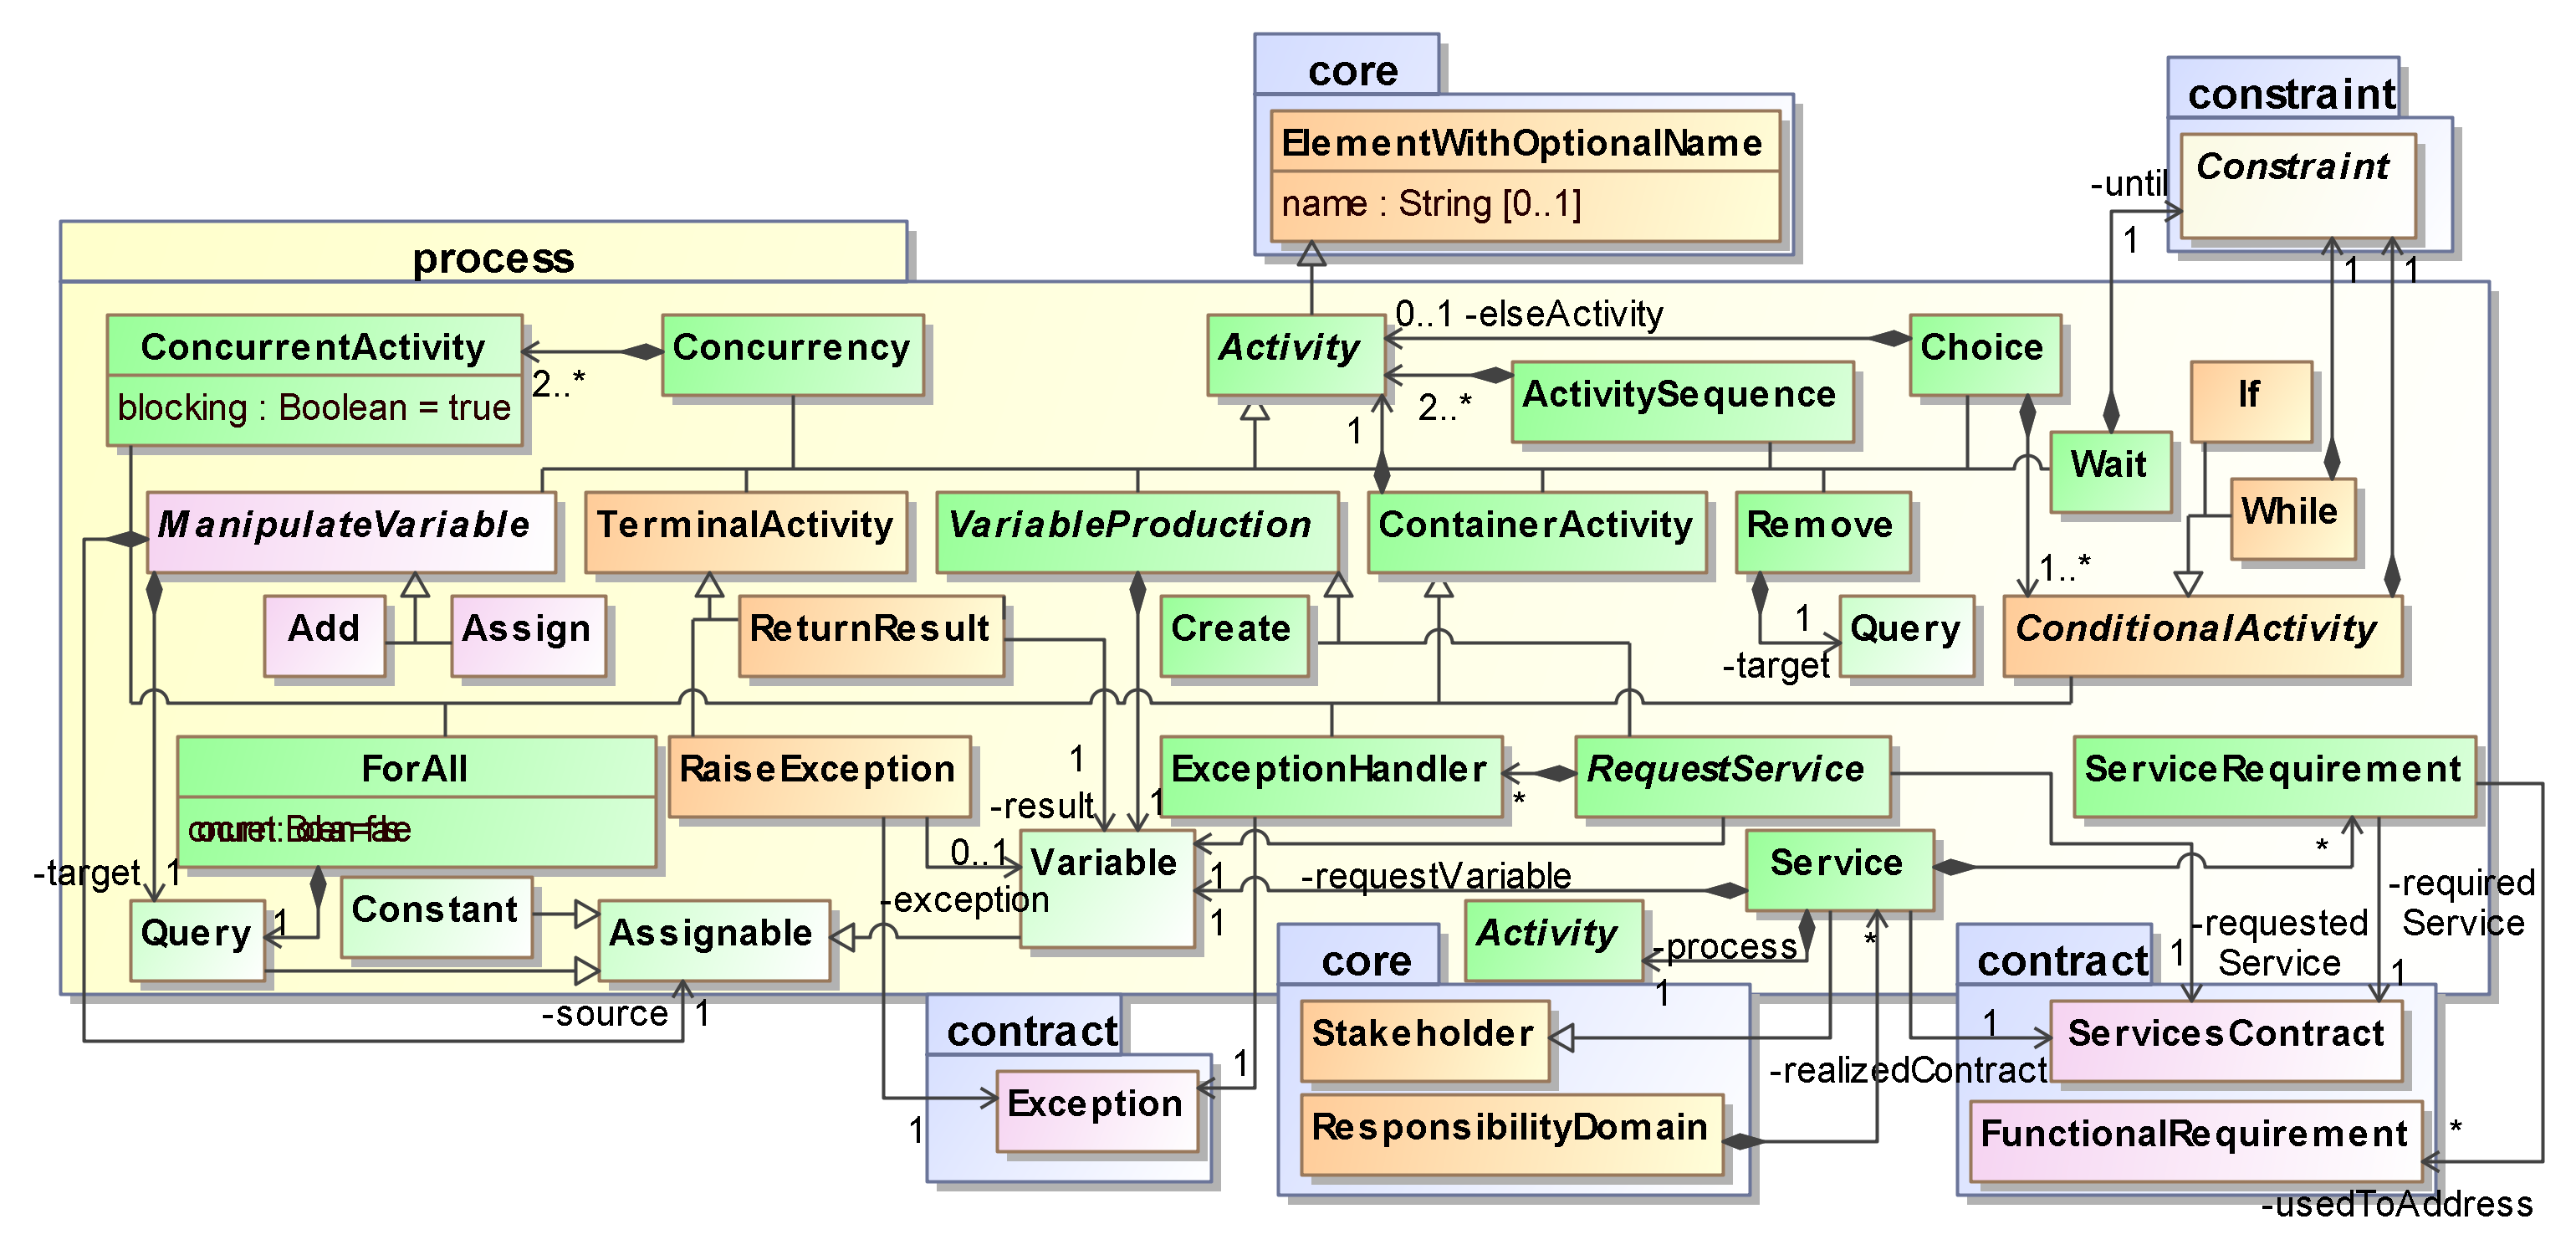
\includegraphics[width=100mm]{process}

\end{frame}

%----------------------------------------------------------------%

\begin{frame}{Syntactic quality drivers}
  Ensure statements made in model comply to syntax rules in metamodel.
  \pause
  \begin{itemize} 
    \item<+-| alert@+> define concrete syntax for encoding of models 
      \begin{itemize}
	\item text-based or diagrammatic
      \end{itemize}
    \item<+-| alert@+> Generate validating editor for concrete syntax.
      \begin{itemize}
	\item Done using MDA tool suite.
      \end{itemize}
    \item<+-| alert@+> Use model validators
      \begin{itemize}
	\item Compliance to metamodel structure.
	\item Adherance to metamodel constraints.
      \end{itemize}
  \end{itemize}
\end{frame}

%----------------------------------------------------------------%

\begin{frame}[fragile]
\frametitle{Example: Service contract specification}

\lstset{language=urdad,label=serviceTextSyntax}
\begin{lstlisting}[numbers=left,escapechar=|]
ResponsibilityDomain RequirementsEngineering
{
  ServiceContract specifyService
  {
    FunctionalRequirements receiving Variable specifyServiceRequest ofType SpecifyServiceRequest
    {
      PreCondition serviceHasStakeholders requiredBy (Client) raises NoStakeholdersException 
       checks Constraint ServiceHasStakeholders
	{
            PreCondition stakeholderRequirementsConsistent requiredBy (Client Implementation Testing) 
		raises InconsistentStakeholderRequirementsException checks Constraint RequirementsConsistent
            PostCondition serviceContractSpecified requiredBy (Client Implementation Testing) 
		ensures Constraint ServiceContractSpecified
            PostCondition processSpecified requiredBy (Client Implementation) ensures Constraint ProcessSpecified
        }
        QualityRequirement traceability requiredBy (ProcessDesign ProjectManagement Development)
        Request DataStructure SpecifyServiceRequest
        {
            has Component serviceRequirements ofType _ServiceRequirements
        }
        Result DataStructure SpecifyServiceResult
        {
            has Component serviceContract ofType _ServiceContract
            has Component service ofType _Service
        }
    }
    Exception NoStakeholdersException {}
    Exception InconsistentStakeholderRequirementsException {}
}
\end{lstlisting}
\end{frame}

%---------------------------------------------------------------%

\begin{frame}{Simplicity quality driver}
  Inverse measure of complexity.
  \begin{itemize} 
    \item<+-| alert@+> Use DSL to provide compact, precise language
      \begin{itemize}
	\item Reduces model size \& understandability.
      \end{itemize}
    \item<+-| alert@+> Ensure all process activities address functional requirements.
      \begin{itemize}
	\item enforced through metamodel.
      \end{itemize}
    \item<+-| alert@+> Enforce single responsibility principle
      \begin{itemize}
	\item Assignment of services to responsibility domains.
      \end{itemize}
    \item<+-| alert@+> No duplication of statements
      \begin{itemize}
	\item Only one way to specify things.
	\item Reuse through enforced adapter layer.
      \end{itemize}
  \end{itemize}
\end{frame}

%---------------------------------------------------------------%

\begin{frame}{Model completeness drivers}
  \begin{itemize} 
    \item<+-| alert@+> Structural completeness criteria
      \begin{itemize}
	\item Enforced through metamodel.
      \end{itemize}
    \item<+-| alert@+>  Process completeness
      \begin{itemize}
	\item All functional requirements addressed.
	\item Enforced through metaodel constraint.
      \end{itemize}
    \item<+-| alert@+> No enforced completeness on levels of granularity.
      \begin{itemize}
	\item Decoupled via services contracts.
	\item Service provider need not be designed - could be plugged in.
      \end{itemize}
    \item<+-| alert@+> Process assistance for completeness via process steps with
      \begin{itemize}
	\item defined inputs \& outputs, and
	\item defined process tasks.
      \end{itemize}
  \end{itemize}
\end{frame}

%---------------------------------------------------------------%

\begin{frame}{Model Consistency Drivers}
  \alert<1>{Consistency often problematic in UML models
    \begin{itemize}
     \item Different UML models structurally and even semantically very different.
     \item Consistency issues across diagrams (e.g. sequence, activity diagrams \& state charts).
    \end{itemize}}
  \pause
  \alert<2>{
  \begin{block}{Model consistency drivers}
    \begin{itemize}
      \item Repeatable process with defined inputs, outputs \& tasks for each process step.
      \item Enforced model structure \& semantics through metamodel.
      \begin{itemize}
	  \item Does not allow duplicate specifications
      \end{itemize}
    \end{itemize}
  \end{block}}
\end{frame}

%---------------------------------------------------------------%

\begin{frame}{Model Cohesion Drivers}
  \begin{itemize}
   \item<+-| alert@+> Responsibility localization
      \begin{itemize}
	\item Contracts contain only services from same responsibility domain.
	\item ``Encouraged'' by process.
      \end{itemize}
   \item<+-| alert@+> Services as cohesive, self-contained units
      \begin{itemize}
	\item Statelessness enforced by metamodel.
	\item Each service must address complete functional requirement at some level of granularity.
      \end{itemize}
  \end{itemize} 
\end{frame}

%---------------------------------------------------------------%

\begin{frame}{Modifiability Drivers}
  \begin{itemize}
   \item<+-| alert@+> Decoupling via services contracts
      \begin{itemize}
	\item Modifiability through decoupling.
	\item ``Enforced'' by process \& metamodel.
      \end{itemize}
   \item<+-| alert@+> Guided levels of granularity
      \begin{itemize}
	\item Process includes step to check whether additional levels of granularity should be defined.
	\item Requirements engineer verifies whether any services at any level of granularity can be combined into single, cohesive, higher-level service.
      \end{itemize}
    \item<+-| alert@+> Simplicity and hence its quality drivers also improve modifiability.
  \end{itemize} 
\end{frame}

%---------------------------------------------------------------%

\begin{frame}{Reusability Drivers}
  \begin{itemize}
   \item<+-| alert@+> All services realize services contracts
      \begin{itemize}
	\item Modifiability through decoupling.
	\item ``Enforced'' by process \& metamodel.
      \end{itemize}
   \item<+-| alert@+> Optimized levels of granularity
      \begin{itemize}
	\item Process includes step to check whether additional levels of granularity should be defined.
	\item Requirements engineer verifies whether any services at any level of granularity can be combined into single, cohesive, higher-level service.
      \end{itemize}
    \item<+-| alert@+> Stateless, self-contained services.
    \item<+-| alert@+> Cohesion and hence its quality drivers also improve discoverability and reusability.
      \note{Discuss example}
    \item<+-| alert@+> Linkage between service and contract it realizes aids service provider discoverability.
  \end{itemize} 
\end{frame}

%---------------------------------------------------------------%

\begin{frame}
  \frametitle{Traceability Drivers}
  Traceability important for validation \& estimation
  \begin{itemize}
   \item Validation for both, sufficiency and necessity.
  \end{itemize}
  \pause
  \begin{block}{Quality drivers}
    \begin{itemize}
      \item<+-| alert@+> Process requires service identification for each functional requirement.
      \item<+-| alert@+> Metamodel provides
	\begin{itemize}
	  \item Traceability of services across levels of granularity.
	  \item Traceability from service to functional requirement realized.
	  \item Traceability from functional requirement to stakeholder who requires it.
	\end{itemize}
    \end{itemize} 
  \end{block}
\end{frame}


%----------------------------------------------------------------%

\begin{frame}[fragile]
\frametitle{Example: Service specification}

\lstset{language=urdad,label=serviceTextSyntax}
\begin{lstlisting}[numbers=left,escapechar=|]
Service specifyServiceImpl realizes specifyService 
	receiving Variable specifyServiceRequest ofType SpecifyServiceRequest
{
    use identifyStakeholders toAddress ( serviceHasStakeholders )
    use performAnalysis toAddress (serviceContractSpecified)
    use designProcess toAddress (processSpecified)

    Process doSequential
    {
	create Variable identifyStakeholdersRequest ofType IdentifyStakeholdersRequest
	set Query OCL:"identifyStakeHoldersRequest.serviceRequirements" 
		equalTo Query OCL:"specifyServiceRequest.serviceRequirements"
	requestService identifyStakeholders with identifyStakeholdersRequest 
		yielding Variable identifyStakeholdersResult ofType IdentifyStakeholdersResult 
		on NoStakeholdersException raiseException NoStakeholdersException

	create Variable specifyServiceContractRequest ofType SpecifyServiceContractRequest
	...
	requestService specifyServiceContract with specifyServiceContractRequest 
		yielding Variable specifyServiceContractResult ofType SpecifyServiceContractResult 
		on InconsistentStakeholderRequirementsException 
			raiseException InconsistentStakeholderRequirementsException
	...
	requestService designProcess with designProcessRequest 
		yielding Variable designProcessResult ofType DesignProcessResult
	
	create Variable specifyServiceResult ofType SpecifyServiceResult
	...
	returnResult specifyServiceResult
    }
}
\end{lstlisting}
\end{frame}

%---------------------------------------------------------------%

\begin{frame}{Testability Drivers}
  \begin{itemize}
    \item<+-| alert@+> Fully specified services contracts
	\begin{itemize}
	  \item In service-oriented paradigm, services can only be tested by
	    \begin{itemize}
	      \item Extracting information about environment using other services.
	      \item Assessing constraints on obtained information.
	    \end{itemize}
	\end{itemize}
    \item<+-| alert@+> Metamodel
	\begin{itemize}
	  \item Contract has constraint as either pre- or post-condition.
	  \item Same state constraint can be pre- and post- condition for different services.
	\end{itemize}
  \end{itemize}
\end{frame}

%----------------------------------------------------------------%

\begin{frame}[fragile]
\frametitle{Example: State constraint specification}

\lstset{language=urdad,label=serviceTextSyntax}
\begin{lstlisting}[numbers=left,escapechar=|]
StateConstraint ServiceContractSpecified receiving Variable serviceRequirements ofType _ServiceRequirements
{
    StateAssessmentProcess doSequential
    {
	create Variable serviceContractAvailable ofType Boolean
	set Query OCL:"serviceContractAvailable" equalTo Constant "true"

	create Variable provideServiceContractRequest ofType ProvideServiceContractRequest
	set Query OCL:"provideServiceContractRequest.serviceRequirements" equalTo 
		Query OCL:"serviceRequirements"
	requestService provideServiceContract with provideServiceContractRequest 
		yielding Variable provideServiceContractResult ofType ProvideServiceContractResult 
		on NoServiceContractAvailableException 
			set Query OCL:"serviceContractAvailable" equalTo Constant "false"
    }
    Constraint OCL:"serviceContractAvailable = true"
}
\end{lstlisting}
\end{frame}
%==========================================================================%

\section{Summary}

\begin{frame}{Summary}
 \begin{itemize}
  \item<+-| alert@+> Different stakeholders in model have overlapping quality requirements.
  \item<+-| alert@+> Process and supporting metamodel has embedded quality drivers.
  \item<+-| alert@+> When using URDAD to design A\&D process, one can regenerate URDAD with its metamodel.
 \end{itemize}
\end{frame}

\end{document}
